%! TEX root = ../thesis.tex
\section{Results}
\label{lmp:sec:results}

\subsection{Baselines}
% - Baseline:
%   - Random
%   - Advanced random -> adapts to the size of conflict
%   - WoW(.) and WoW(R)
% - Introduce the WoW model (starting from the previous paper); this model will serve as a baseline.
%   - We adopt the terminology of us et al.

We start by introducing the baselines against which we compare our models.
For each baseline and for our models, we assume a set of~$K$ conflicting edits \mbox{$\mathcal{C} = \{ a, b, \ldots \}$} proposed on dossier~$i$, for which we want to model the probability that an edit~$a \in \mathcal{C}$ is accepted over edits~$b, \ldots$ on this dossier.
We denote this probability by~$\Prob{ a \succ_i \mathcal{C} - \{ a\} }$, and we denote the probability that the status quo wins, \textit{i.e.}, that the original text proposed by the Commission is kept, by~$\Prob{ i \succ \mathcal{C} } = 1 - \sum_{a\in \mathcal{C}} \Prob{ a \succ_i \mathcal{C} - \{a\} }$.

\paragraph{Naive Classifier}

The \textit{naive classifier} predicts a uniform probability for each outcome, \textit{i.e.}, for each of the conflicting edits or the status quo to win, as
\begin{equation*}
	\Prob{ a \succ_i \mathcal{C} - \{ a\} } = \Prob{ i \succ \mathcal{C} } = \frac{1}{K + 1}.
\end{equation*}

\paragraph{Random Classifier}

The \textit{random classifier} learns the prior probability~$p^{(K)}$ that the status quo wins for each conflict size~$\vert \mathcal{C} \vert = K$, and it predicts
\begin{equation*}
	\Prob{ i \succ \mathcal{C} } = p^{(K)}.
\end{equation*}
It predicts uniformly each of the edits to win as
\begin{equation*}
	\Prob{ a \succ_i \mathcal{C} - \{ a\} } = \frac{1-p^{(K)}}{K}.
\end{equation*}

\subsection{Experimental Setting}

% Explain the metrics we use for evaluation.
We report the cross-entropy loss to evaluate the baselines and our models.
Let~$( \mathcal{C}_n, i_n, l_n )$ be an observation.
We compute
\begin{equation}
	\ell_n = \begin{cases}
		-\log \Prob{l_n \succ_{i_n} \mathcal{C}_n - \{l_n\} } & \text{if $l_n \in \mathcal{C}_n$}, \\
		-\log \Prob{i_n \succ \mathcal{C}_n}                  & \text{if $l_n = i_n$}.
	\end{cases}
\end{equation}
We report the average value for all~$N$ points in our test set as~$\ell = \frac{1}{N} \sum_n \ell_n$.
%, and we compute the 99\% confidence intervals around this average.
% - Explain the training and testing procedure
% - Explain how we chose the best hyperparameters
We randomize our dataset and we split it into 80\% for training, 10\% for validation, and 10\% for the final evaluation.
We combine both the training and the validation sets to fit our model before evaluating it on the test set.
We set the number of latent dimensions~$L$ and the regularizers, and we choose the best word embeddings, by held-out validation.
% Please refer to Appendix~\ref{app:hyperparameters} for a complete list of the best hyperparameters that we used.
This results in fastText of dimension~$D = D' = 10$, with bigrams.

\subsection{Predictive Performance}
% - Give and discuss the predictive performance of all models
%   - Predicting a new edit
% - Plot the results in terms of
%   - Log-loss
%   - Accuracy?
%   - F1-Score/AUC?

We show in Figure~\ref{lmp:fig:results} the overall performance of all variations of our model (with and without explicit, latent, and text features) over EP7 and EP8, and we compare them against the naive and the random predictors, as well as against the \wow{} model.
All our models outperform the baselines, and \wow{XLT} outperforms all other models.
Including explicit features improves the performance of the predictions in terms of the cross entropy by 6\% for EP7 and 5\% for EP8 over the simpler \wow{} model.
Similarly, \wow{L} and \wow{T} further improves the performance over \wow{} by 14\% for EP7 and by 12\% for EP8.
Hence, the text and latent features provide a greater improvement than the explicit features.
Combining the text and latent features provides high performance, but further combining them with explicit features leads to the best performance.
The difference between \wow{XL} and \wow{L} (0.007 for EP7 and 0.009 for EP8) is less than the difference between \wow{XT} and \wow{T} (0.024 for bot EP7 and EP8), as the latent features absorb the effects of the explicit features more than the text features do.

\begin{figure}
  \centering
  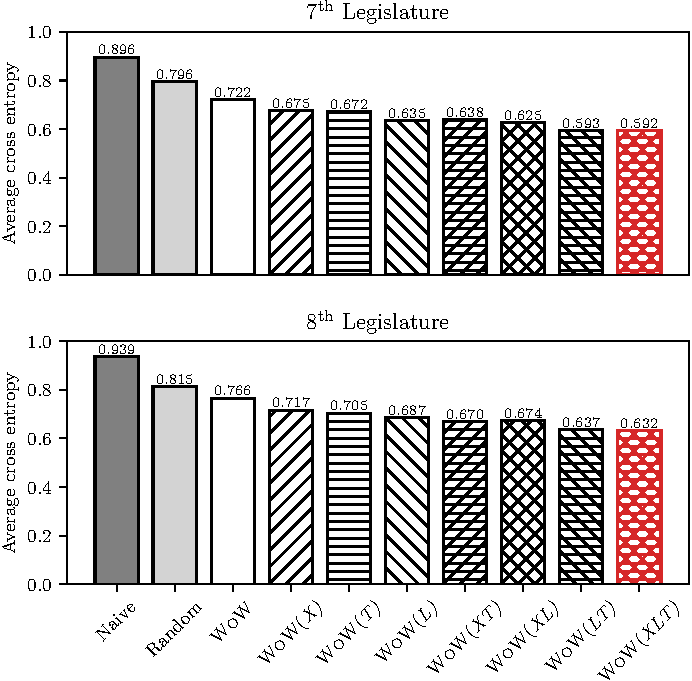
\includegraphics[width=\linewidth*3/4]{lmp-results}
	\caption{%
		Average cross-entropy loss of the baselines and our models.
		Combining the explicit, latent, and text features help obtain the best performance.
	}
	\label{lmp:fig:results}
\end{figure}

% Move to a new section?
\subsection{Interpretation of Explicit Features}

% - Explore the contribution of different explicit features to the performance of the model
To understand the contribution of the explicit features to the predictive performance, we show in Figure~\ref{lmp:fig:improvement} the decrease in cross-entropy loss of \wow{MEP} (all MEP features but the rapporteur feature), \wow{Rapp.} (rapporteur feature only), \wow{Edit}, and \wow{Dossier} over \wow.
The dossier features contribute virtually nothing to the predictive performance (the difference is at the fourth decimal point).
Similarly, for EP7, the nationality, political group, and gender features of \wow{MEP} contribute very little.
For EP8, these features improve the performance, but not as much as the edit features.
This suggests that these features have limited influence on the predictions.
Nationalities and political groups have been qualitatively analyzed in the literature in the context of their influence on MEPs' voting behaviour~\cite{hix2002parliamentary,coman2009reassessing,muhlbock2012national,lefkofridi2014multilevel}.
To the best of our knowledge, there is no analysis of their effect on the amending process.
Interestingly, for EP7, combining all features into the \wow{X} model leads to a performance boost that is greater than the sum of each individual feature groups.

\begin{figure}
  \centering
  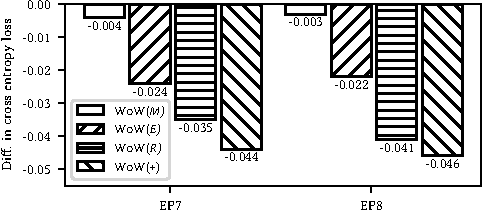
\includegraphics[width=\linewidth*3/4]{lmp-improvement}
	\caption{%
		Difference in cross-entropy loss over \wow{} of different models.
		The rapporteur feature and the edit features contribute more to the predictive performance than the MEP and dossier features.
	}
	\label{lmp:fig:improvement}
\end{figure}

\paragraph{Contribution of Explicit Features}

Let~$w_f \in \mathbf{R}$ be the value of the parameter associated with feature~$f$.
The rapporteur feature~$r$ of \wow{Rapp.} provides a greater decrease in loss.
This \textit{rapporteur advantage} complements the findings of~\citet{costello2010policy}, conducted by interviewing key informants over EP5 (1999-2004) and EP6 (2004-2009).
They show that the rapporteur, with their particular role, has some influence on the legislative process, albeit constrained.
We note that, according to our model, the rapporteur advantage has slightly increased in EP8 ($w_r=1.12$) compared to EP7 ($w_r=1.11$).

% - Interpret the values that different parameter of the explicit features take
These explicit features enable us to explain what contributes to the success of an edit.
We report here (and in subsequent sections) the results for EP8 only.
All other things being equal, a female ($w_{\text{fem}}=0.02 > -0.04 = w_{\text{mal}}$) MEP from Luxembourg and whose party belongs to the Alliance of Liberals and Democrats (center) has the highest chance to see her edit accepted.
This edit has even higher chances if it inserts ($w_{\text{ins}}=-0.02 > w_{\text{del}}=-0.11 > w_{\text{rep}}=-0.23$) a short portion of text (the feature associated with both insertion and deletion length is negative) in a part of the law that is not its body or its preamble ($w_{\text{art}}$ and~$w_{\text{rec}}$ have the lowest value among the seven article types).
Adding a justification also increases the probability of an edit being accepted ($w_{\text{jus}}=0.09$), as well as edits from the opinion committee (referred to as the "outsider committee" feature in Table~\ref{lmp:tab:features},~$w_{\text{out}} =  0.07$).

For the dossier features, our model learns that it is harder to make edits on reports, as compared to opinions (($w_{\text{rep}}=0.41 > -0.40 = w_{\text{opi}}$)).
As explained in Section~\ref{lmp:sec:dataset}, reports are voted by the whole Parliament.
Therefore, they have a greater influence on the final law, and we expect that MEPs make it more difficult for competing edits to be accepted in reports.
Surprisingly, our model also learns that it is harder to make edits for decisions (the legal acts that are binding for one member state only), as compared to regulations and directives ($w_{\text{dec}}=0.14 > 0.10 = w_{\text{reg}} = w_{\text{dir}}$).

\paragraph{Controversy of Dossiers}

Table~\ref{lmp:tab:inertia_params} provides a list of the three dossiers in EP8 with the highest inertia parameter~$d_i$ and the three dossiers with the lowest~$ d_i $.
The values of $d_i$ correlate well with the number of nodes, the number of cliques, the average size of cliques, and the edit acceptance rate.
The top-three dossiers include laws with high stakes:
The "Screening of foreign direct investments" sets a framework to better equip the EU for investments from non-EU countries.
It has crucial implications for companies, workers, governments, and citizens.
The infamous "Copyright in the Digital Single Market", considered to be a threat to freedom of expression on the Web by its opponents, sparked public protests in several cities.
The reporting committee publicized that "MEPs have rarely or never been subject to a similar degree of lobbying before"\cite{europarl2019questions}.
Finally, the "Energy efficiency labelling" updated famous labels for electrical appliances, which guide consumers in their purchases.

The number of nodes, the number of cliques, the average size of cliques, and the percentage of accepted edits correlate with the value of parameter~$ d_i$.
These four metrics are a good proxy to the level of activity by MEPs in the amending process of a given dossier.
Higher activity, possibly due to higher controversy, leads to higher value of~$d_i$.
Similarly, the skill parameters~$s_u$ enable us to quantify the influence of each MEP.
The value of~$s_u$ increases the most when MEP~$u$ wins against stronger MEPs and on dossier~$i$ with high inertia~$d_i$.
The number of edits, the proportion of successful edits, and the proportion of successful conflicts correlate with the value of parameter~$s_u$ (not shown here for space constraints).
A MEP able to propose many edits with high acceptance rate, has their political views strongly represented in laws.

% \begin{table}
%   \centering
% 	\caption{Top-3 and bottom-3 dossiers in EP8 according to their inertia parameters $d_i$.}
% 	\label{lmp:tab:inertia_params}
% 	\begin{tabular}{rllrrrr}
% 		\toprule
% 		$d_i$  & Type    & Title                                                         & \# nodes & \# cliques & avg. clique size & \% accepted \\
% 		\midrule

% 		3.304  & report  & Screening of foreign direct investments                       & 1040     & 272        & 3.1              & 2.6         \\
% 		3.204  & report  & Copyright in the Digital Single Market                        & 2657     & 577        & 4.3              & 2.6         \\
% 		3.106  & report  & Energy efficiency labelling                                   & 1292     & 319        & 3.4              & 6.0         \\

% 		\midrule

% 		-2.611 & opinion & Financial support for customs control equipment               & 60       & 1          & 2.0              & 90.0        \\
% 		-2.644 & opinion & Establishing the supervisory authorities on financial markets & 69       & 0          & 0.0              & 98.6        \\
% 		-2.849 & opinion & Unfair trading practices in the food supply chain             & 63       & 6          & 2.0              & 84.1        \\

% 		\bottomrule
% 	\end{tabular}
% \end{table}he bottom-three dossiers are all opinions, which are intrinsically less important than reports, as explained in Section~\ref{lmp:sec:background}.

% TODO: Update this table with the correct top-5 and bottom-5.
\begin{sidewaystable}
  \centering
  \caption{Inertia parameters~$d_i$ for dossiers in EP8.}
  \label{lmp:tab:inertia_params}
  \begin{tabular}{rllrrrr}
    \toprule
    $d_i$ & Type & Title & \# edits & \# conf. & avg.\ conf. size & \% accepted \\
    \midrule

    2.055 & opinion & Cost-effective emission reductions             & 1756 & 385 & 4.2 & 5.1\% \\
    1.502 & report  & Copyright in the Digital Single Market         & 2657 & 577 & 4.3 & 2.6\% \\
    1.324 & report  & Screening of foreign investments into the EU   & 1040 & 272 & 3.1 & 2.6\% \\
    1.308 & report  & Specific programme implementing Horizon Europe & 2886 & 654 & 2.7 & 13.1\% \\
    1.272 & report  & Rules of participation in Horizon Europe       & 2013 & 467 & 3.0 & 9.8\% \\

    \midrule

    -0.829 & report  & Complementing the Criminal Records Information System & 246 & 56 & 2.2 & 41.9\% \\
    -0.864 & opinion & Financial information for the detection criminals     & 81  & 2  & 2.0 & 86.4\% \\
    -0.936 & report  & Establishing a Community Code on Visas                & 259 & 61 & 2.2 & 47.5\% \\
    -0.949 & opinion & Rules of participation in Horizon Europe              & 198 & 36 & 2.2 & 58.6\% \\
    -1.445 & report  & Financial rules to the general budget of the EU       & 650 & 13 & 2.0 & 86.9\% \\

    \bottomrule
  \end{tabular}
\end{sidewaystable}

\subsection{Interpretation of Text Features}
\label{lmp:sec:intertext}

In Figure~\ref{lmp:fig:results}, we observe that the text features contribute significantly to improving the performance.
We use the learned parameter vectors~$\boldsymbol{w}_T$ and~$\boldsymbol{w}_{T'}$ of \wow{XLT} to identify words and bigrams that have the most predictive power.
First, we rank the words and bigrams of the edit text, according to the dot product of their embeddings with~$\boldsymbol{w}_T$.
The top-$k$ terms (having a positive dot product) contribute the most towards acceptance of the edit, whereas the bottom-$k$ terms (having a negative dot product) contribute most towards rejection of the edit.
The opposite holds for the terms of the title and their dot product with~$\boldsymbol{w}_{T'}$.

We look at the top~$50$ terms for each feature and prediction outcome and find some interesting patterns among these terms, although not all of them are easy to interpret.
Note that we have more than~\numprint{10000} unique terms for the edit text and more than~\numprint{1000} unique terms for the title, hence we consider only the most predictive terms near the ends of the ranking.
% A list of the top-50 terms for each feature and prediction outcome is reported in Appendix~\ref{app:accept}.

%We first examine the words and bigrams in the inserted and deleted text are predictive of acceptance.
%We see the word \textit{consumer} here, which commonly occurs in laws on consumer rights.
%This suggests that deleting provisions of the laws that give rights or benefits to consumers might be getting accepted often (possibly under the influence of lobbies), and indeed we see many such examples in the dataset.
One of the bigrams that, when deleted, is predictive of acceptance is \textit{any other}, which is commonly used to widen the scope of the law (as in ``contractual or any other duty'').
The word \textit{should}, which is used to add recommendations, is predictive of acceptance when inserted.
Adding \textit{must} and \textit{binding}, which are used for obligations, are predictive of rejection.
We see that \textit{best} is predictive of acceptance, which is commonly used to make a requirement stronger (as in ``best available scientific evidence'', ``best possible way'').
Adding \textit{positive} and \textit{positive impact} predicts acceptance, whereas adding \textit{negative} predicts rejection.
Adding the word \textit{inserted}, which commonly refers to inserting new articles in existing laws, is predictive of acceptance, whereas \textit{deleted} is predictive of rejection.

Considering the words in the context, we see that \textit{firearms}, \textit{resettlement} and \textit{privacy} are predictive of rejection.
This could be because the laws related to these topics are controversial, hence many edits are rejected due to conflicts.
For the words in the title, we see that \textit{customs}, \textit{community}, \textit{medicines}, and \textit{general budget} are predictive of acceptance, whereas \textit{market}, \textit{framework}, \textit{structural reform}, \textit{emission},  and \textit{greenhouse gas} are predictive of rejection.
This suggests the relative ease or difficulty of editing laws related to these topics, and it correlates well with the values of the difficulty parameters~$d_i$:
The top-10 dossiers with the highest difficulty parameters contain high-controversy dossiers about the screening of foreign investments, the regulation of the financial market, vast public investment programs (InvestEU), and  carbon-emission reduction and low-carbon investments,
The bottom-10 dossiers with the lowest difficulty parameters contain low-controversy dossiers about frequency bands, the attribution of the general budget to border protection and cohesion within the EU, accessibility requirements, and the information systems of criminal records.

\subsection{Interpretation of Latent Features}
% - Interpretation of the latent features
%   - In terms of ideological space for the dossier and the MEPs
%   - Explains why they improve the performance, by capturing different ideologies rather than explicit party assignment

The latent features improve the predictions overall and help capture the complex dynamics of the legislative process.
The best number of latent dimensions is~$L = 10$  for the \wow{XLT} and the \wow{LT} models, and it is~$L = 20$ for \wow{L} and \wow{XL}.
In order to interpret the latent features, we gather the latent vectors~$\bm{y}_i$ learned by \wow{XLT} into a matrix~$Y = [ \bm{y}_i ]$.
We apply principal component analysis and keep the top-10 and bottom-10 dossiers from each of the first two principal components in EP8.
We use t-SNE~\cite{maaten2008visualizing} to represent these forty dossiers in a two-dimensional space, and we show the projection in Figure~\ref{lmp:fig:tsne}.

We distinguish four clusters.
The cluster at the top contains dossiers about investment and development programmes, finance and digitalization, and sustainable development.
We interpret this cluster as \textit{investment and development}, and we highlight with blue dots the corresponding dossiers.
The cluster at the right contains dossiers about retirement, refugees, protection of consumer and workers, and limitation of financial risk.
We interpret this cluster as \textit{social security} (green triangles).
The cluster at the bottom contains dossiers about support of the defense industry and the establishment of defense funds.
It also contains dossiers about protection of workers against pollutants, international and financial protection, and rules of accession to the EU.
We interpret this cluster as \textit{defense and protection} (red crosses).
Finally, the cluster at the left contains dossiers about economic development, innovation, and businesses, as well as dossiers about unfair trading, trade secrets, and the screening of foreign investments.
We interpret this cluster as \textit{economic competitiveness} (blue dots).

\begin{figure}
  \centering
  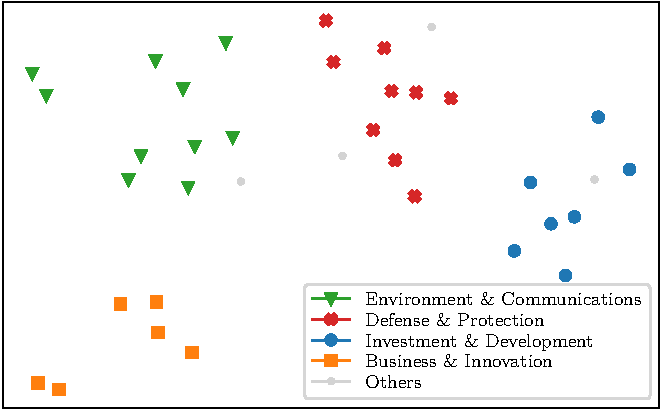
\includegraphics[width=\linewidth*3/4]{lmp-tsne}
	\caption{Visualization with t-SNE of the top-10 and bottom-10 dossiers on the first two principal components in EP8.}
	\label{lmp:fig:tsne}
\end{figure}

\subsection{Error Analysis by Conflict Size}
% - Compute the performance of high- and low-controversy dossiers
%   - Dynamics of law-making is different depending of the level of controversy
%   - We can not use the same predictor, but the hybrid models bridges the gap
% - Compute performance per committees
% - Compute performance per topic

We explore how the \wow{XLT} model performs on conflict of different sizes in the test set for EP8 (we observe a similar behaviour on EP7).
We bin the conflict size so that there are at least 100 data points in each bin.
The distribution of conflict size is exponentially decreasing:
There are 8423 conflicts of size 1 (\textit{i.e.}, an edit is in conflict with the status quo only), 3089 conflicts of size 2 (\textit{i.e.}, two edits are in conflict, as well as with the status quo),  and 107 conflicts of size 8 and more.
We compare the average cross entropy of the \wow{XLT} model with that of the random predictor and that of the \wow{} model.
In Figure~\ref{lmp:fig:error-analysis}, the loss of \wow{XLT} increases less rapidly with conflicts of larger sizes than the two baselines.
This suggests that the explicit, latent, and text features enable the model to exploit the increasing complexity of data points to make more accurate predictions.
The drop in entropy for conflicts of size 8 and more may be due to the low number of data points in this bin.

\begin{figure}
  \centering
  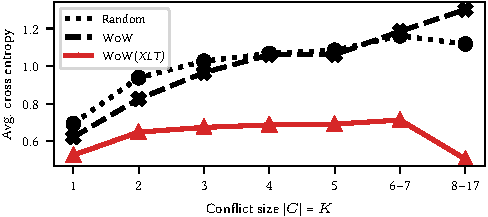
\includegraphics[width=\linewidth*3/4]{lmp-error-analysis}
	\caption{%
		Average cross-entropy loss per conflict size~$\vert \mathcal{C} \vert = K$.
		The loss of the \wow{XLT} model increases less rapidly than the loss of the baselines.
	}
	\label{lmp:fig:error-analysis}
\end{figure}

\subsection{Solving the Cold-Start Problem}
\label{lmp:sec:cold-start}

% - Predicting an edit for a new dossier
We explore how to solve the cold-start problem by defining a second predictive problem:
Given a dossier~$i$ \textit{for which we have never seen an edit}, and given a conflict~$\mathcal{C} = \{a, b, \ldots \}$, we want to predict which of the edits or the status quo wins.
We order the dossiers by the date a committee received a proposal, and we use the dossiers that contain the first 80\% of the conflicts as a training set.
We use the next 10\% as validation set, and we keep the last 10\% aside as test set.
We ensure that no edits in the training set leak into the validation and test sets.
This scenario is more realistic because we make predictions about new dossiers that the model has never observed before.

We report, in Table~\ref{lmp:tab:newdossier}, the results for \wow{Explicit}, \wow{Text}, and \wow{XT}, together with the baselines.
The latent features cannot be used for this task, as the dossier embeddings~$\vec{y}_i$ are unavailable for new dossiers.
For our models, the difficulty parameter~$d_i$ is set to the average difficulty learned in the training set.
The random predictor, which learns the prior probability of the status quo winning for each conflict size, performs the best out of all the baselines, and it outperforms \wow{Text}.
Our approach outperforms only the random predictor when including explicit features.
This suggests that the dossier features help us make more accurate predictions by learning parameter values for the type of dossier, its legal act, and its committee in charge.
In this case, adding text features further boosts the performance.

The overall performance, however, is mixed:
The improvement of \wow{XT} over the random predictor is rather small.
One possible explanation is that the legislative process might be non-stationary.
Hence, our model overfits on the training set, which is very different from the test set.
The task is also unfair to our model, as in a real setting, predictions would be made for the next dossier only.
In the current setting, we make predictions for all future dossiers.
We keep further investigations of this aspect for future work.

\begin{table}
  \centering
	\caption{Average cross entropy of the baselines and our model on predicting new, unseen dossiers.}
	\label{lmp:tab:newdossier}
	\begin{tabular}{llr}
		\toprule
		Type     & Model          & Avg.\ cross entropy \\
		\midrule
		Baseline & Naive          & 0.947               \\
		         & Random         & \textbf{0.800}      \\
		         & \wow{}       & 0.873               \\
		\midrule
		Ours     & \wow{Explicit} & 0.784               \\
		         & \wow{Text}     & 0.839               \\
		         & \wow{XT}       & \textbf{0.759}      \\
		\bottomrule
	\end{tabular}
\end{table}
